\documentclass[../master_galois_theory]{subfiles}
\begin{document}

\setcounter{section}{13}

\section{Galois cohomology}

\subsection{群のcohomology}

\begin{defi} \label{defi:cochain}
  $G:$群、 $M:$加法 $(\mathrm{Abel})$群で
  $G$は $M$に加群としての作用をしているとする。
  ここで以下のように $G^n$から $M$への写像全体の集合を
  $C^n (n \in \Z_{\geq 0})$として定める。
  \begin{eqnarray*}
    C^n = C^n(G,M) := \{ f : G^n \longrightarrow M \} = \map(G^n,M)
  \end{eqnarray*}
  ただし $G^0 = \{ e \}$と考えることで $C^0 := M$と定める。
  この $C^n$の各元を\underline{ $n$コチェイン $(\mathrm{cochain})$}という。
  $C^n$上へは $f , g \in C^n$に対して
  $(f+g)(x) := f(x) + g(x)$と演算を定めることで $C^n$は加法群となる。
\end{defi}

\begin{defi} \label{defi:coboundary}
  $C^n$から $C^{n+1}$への以下のように定まる写像 $\partial$を考える。
  \begin{eqnarray*}
    \partial = \partial^n : C^n & \longrightarrow & C^{n+1} \\
    f & \longmapsto & \partial f
  \end{eqnarray*}
  ここで $\partial f : G^{n+1} \longrightarrow M$は
  $G$が $M$へ作用していることに注意して
  \begin{eqnarray*}
    \partial f(g_1 , \dots , g_{n+1}) & = & g_1 f(g_2 , \dots , g_{n+1}) \\
    & + & \sum_{i=1}^n (-1)^i f(g_1 , \dots , g_i g_{i+1} , \dots , g_{n+1}) \\
    & + & (-1)^{n+1} f(g_1 , \dots , g_n)
  \end{eqnarray*}
と定める。
このときこの $\partial (= \partial^n) : C^n(G,M) \longrightarrow C^{n+1}(G,M)$は加法群の準同型になり、
これを\underline{$n$次のコバウンダリー $(双対境界)$作用素 $(\mathrm{coboundary \  operator})$}とよぶ。
\end{defi}

\begin{prop} \label{prop:partialpartial}
  コバウンダリー作用素 $\partial$に対して $\partial^{n+1} \circ \partial^n = 0$が成り立つ。
\end{prop}

\begin{proof}
  $4 \leq n$でまず考える。

  $(\partial^{n+1} \circ \partial^n)(f)(g_1 , \dots , g_{n+2}) = \partial^{n+1}(\partial^n f)(g_1 , \dots , g_{n+2})$なので
  $f' := \partial^n f$として $\partial^{n+1}f'(g_1 , \dots , g_{n+2})$は
  \begin{eqnarray*}
    \partial^{n+1}f'(g_1 , \dots , g_{n+2}) & = & g_1 f'(g_2 , \dots , g_{n+2}) \\
    & + & \sum_{i=1}^{n+1} (-1)^i f'(g_1 , \dots , g_i g_{i+1} , \dots , g_{n+2}) \\
    & + & (-1)^{n+1} f'(g_1 , \dots , g_{n+1})
  \end{eqnarray*}
  である。
  $f'(g_1 , \dots , g_i g_{i+1} , \dots , g_{n+2}) = \partial^n f(g_1 , \dots g_i g_{i+1} , \dots , g_{n+2})$を $i$の値によって計算する。

  ・ $i = 1$のとき
  \begin{eqnarray*}
    \partial^n f(g_1 g_2 , \dots ,g_{n+2}) & = & g_1 g_2 f(g_3 , \dots , g_{n+2}) \\
    & + & (-1)^1 f((g_1 g_2) g_3 , g_4 , \dots , g_{n+2}) \\
    & + & \sum_{k=3}^{n+1} (-1)^{k-1} f(g_1 g_2 , g_3 , \dots , g_i g_{i+1} , \dots , g_{n+2}) \\
    & + & (-1)^{n+1} f(g_1 g_2 , g_3 , \dots , g_n)
  \end{eqnarray*}
  ・ $i = 2$のとき
  \begin{eqnarray*}
    \partial^n f(g_1 , g_2 g_3 , g_4 , \dots , g_{n+2}) & = & g_1 f(g_2 g_3 , g_4 , \dots , g_{n+2}) \\
    & + & (-1)^1 f(g_1 (g_2 g_3) , g_4 , \dots , g_{n+2}) \\
    & + & (-1)^2 f(g_1 , (g_2 g_3) g_4 , g_5 , \dots , g_{n+2}) \\
    & + & \sum_{k=4}^{n+1} (-1)^{k-1} f(g_1 , g_2 g_3 , g_4 , \dots , g_i g_{i+1} , \dots , g_{n+2}) \\
    & + & (-1)^{n+1} f(g_1 , g_2 g_3 , g_4 , \dots , g_{n+1})
  \end{eqnarray*}
  ・ $3 \leq i \leq n-1$のとき
  \begin{eqnarray*}
    \partial^n f(g_1 , \dots , g_i g_{i+1} , \dots , g_{n+2}) & = & g_1 f(g_2 , \dots , g_i g_{i+1} , \dots , g_{n+2}) \\
    & + & \sum_{k=1}^{i-2} (-1)^k f(g_1 , \dots , g_k g_{k+1} , \dots , g_i g_{i+1} , \dots , g_{n+2}) \\
    & + & (-1)^{i-1} f(g_1 , \dots , g_{i-2} , g_{i-1} (g_i g_{i+1}) , g_{i+2} , \dots , g_{n+2}) \\
    & + & (-1)^i f(g_1 , \dots , g_{i-1} , (g_i g_{i+1}) g_{i+2} , g_{i+3} , \dots , g_{n+2}) \\
    & + & \sum_{k=i+2}^{n+1} (-1)^{k-1} f(g_1 , \dots , g_i g_{i+1} , \dots , g_k g_{k+1} , \dots , g_{n+2}) \\
    & + & (-1)^{n+1} f(g_1 , \dots , g_i g_{i+1} , \dots , g_{n+1})
  \end{eqnarray*}
  ・ $i = n$のとき
  \begin{eqnarray*}
    \partial^n f(g_1 , \dots , g_n g_{n+1} , g_{n+2}) & = & g_1 f(g_2 , \dots , g_n g_{n+1} , g_{n+2}) \\
    & + & \sum_{k=1}^{n-2} (-1)^k f(g_1 , \dots , g_k g_{k+1} , \dots , g_n g_{n+1} , g_{n+2}) \\
    & + & (-1)^{n-1} f(g_1 , \dots , g_{n-1} (g_n g_{n+1}) , g_{n+2}) \\
    & + & (-1)^n f(g_1 , \dots , g_{n-1} , (g_n g_{n+1}) g_{n+2}) \\
    & + & (-1)^{n+1} f(g_1 , \dots , g_{n-1} , g_n g_{n+1})
  \end{eqnarray*}
  ・ $i = n+1$のとき
  \begin{eqnarray*}
    \partial^n f(g_1 , \dots , g_{n+1} g_{n+2}) & = & g_1 f(g_2 , \dots , g_{n+1} g_{n+2}) \\
    & + & \sum_{k=1}^{n-1} (-1)^k f(g_1 , \dots , g_k g_{k+1} , \dots , g_n , g_{n+1} g_{n+2}) \\
    & + & (-1)^n f(g_1 , \dots , g_{n-1} , g_n (g_{n+1} g_{n+2})) \\
    & + & (-1)^{n+1} f(g_1 , \dots , g_n)
  \end{eqnarray*}
となる。

また、 $g_1 f'(g_2 , \dots , g_{n+2})$と $(-1)^{n+2} f'(g_1 , \dots , g_{n+1})$は以下のようになる。
\begin{eqnarray*}
  g_1 \partial^n f(g_2 , \dots , g_{n+2}) & = & g_1 (g_2 f(g_3 , \dots , g_{n+2}) \\
  & + & \sum_{i=2}^{n+1} (-1)^{i-1} f(g_2 , \dots , g_i g_{i+1} , \dots , g_{n+2}) \\
  & + & (-1)^{n+1} f(g_2 , \dots , g_{n+1}) ) \\
  (-1)^{n+2} \partial^n f(g_1 , \dots , g_{n+1}) & = & (-1)^{n+2} (g_1 f(g_2 , \dots , g_{n+1}) \\
  & + & \sum_{i=1}^n (-1)^i f(g_1 , \dots , g_i g_{i+1} , \dots , g_{n+1}) \\
  & + & (-1)^{n+1} f(g_1 , \dots , g_n) )
\end{eqnarray*}

これを $\partial^{n+1}(\partial^n f)(g_1 , \dots , g_{n+2})$の式に代入すると
\begin{eqnarray*}
  \partial^{n+1}(\partial^n f)(g_1 , \dots , g_{n+2}
  % g_1 f'(g_2 , \dots , g_{n+2})
  & = & \{ g_1 g_2 f(g_3 , \dots , g_{n+2}) \\
  & + & \sum_{i=2}^{n+1} (-1)^{i-1} g_1 f(g_2 , \dots , g_i g_{i+1} , \dots , g_{n+2}) \\
  & + & (-1)^{n+1} g_1 f(g_2 , \dots , g_{n+1}) \} \\
  % i = 1
  & + & (-1)^1 \{ g_1 g_2 f(g_3 , \dots , g_{n+2}) \\
  & + & (-1)^1 f((g_1 g_2) g_3 , g_4 , \dots , g_{n+2}) \\
  & + & \sum_{k=3}^{n+1} (-1)^{k-1} f(g_1 g_2 , g_3 , \dots , g_i g_{i+1} , \dots , g_{n+2}) \\
  & + & (-1)^{n+1} f(g_1 g_2 , g_3 , \dots , g_n) \} \\
  % i = 2
  & + & (-1)^2 \{ g_1 f(g_2 g_3 , g_4 , \dots , g_{n+2}) \\
  & + & (-1)^1 f(g_1 (g_2 g_3) , g_4 , \dots , g_{n+2}) \\
  & + & (-1)^2 f(g_1 , (g_2 g_3) g_4 , g_5 , \dots , g_{n+2}) \\
  & + & \sum_{k=4}^{n+1} (-1)^{k-1} f(g_1 , g_2 g_3 , g_4 , \dots , g_i g_{i+1} , \dots , g_{n+2}) \\
  & + & (-1)^{n+1} f(g_1 , g_2 g_3 , g_4 , \dots , g_{n+1}) \} \\
  % 3 \leq i \leq n-1
  & + & \sum_{i=3}^{n-1} (-1)^i \{ g_1 f(g_2 , \dots , g_i g_{i+1} , \dots , g_{n+2}) \\
  & + & \sum_{k=1}^{i-2} (-1)^k f(g_1 , \dots , g_k g_{k+1} , \dots , g_i g_{i+1} , \dots , g_{n+2}) \\
  & + & (-1)^{i-1} f(g_1 , \dots , g_{i-2} , g_{i-1} (g_i g_{i+1}) , g_{i+2} , \dots , g_{n+2}) \\
  & + & (-1)^i f(g_1 , \dots , g_{i-1} , (g_i g_{i+1}) g_{i+2} , g_{i+3} , \dots , g_{n+2}) \\
  & + & \sum_{k=i+2}^{n+1} (-1)^{k-1} f(g_1 , \dots , g_i g_{i+1} , \dots , g_k g_{k+1} , \dots , g_{n+2}) \\
  & + & (-1)^{n+1} f(g_1 , \dots , g_i g_{i+1} , \dots , g_{n+1}) \} \\
  % i = n
  & + & \{ g_1 f(g_2 , \dots , g_n g_{n+1} , g_{n+2}) \\
  & + & \sum_{k=1}^{n-2} (-1)^k f(g_1 , \dots , g_k g_{k+1} , \dots , g_n g_{n+1} , g_{n+2}) \\
  & + & (-1)^{n-1} f(g_1 , \dots , g_{n-1} (g_n g_{n+1}) , g_{n+2}) \\
  & + & (-1)^n f(g_1 , \dots , g_{n-1} , (g_n g_{n+1}) g_{n+2}) \\
  & + & (-1)^{n+1} f(g_1 , \dots , g_{n-1} , g_n g_{n+1}) \} \\
  % i = n+1
  & + & \{ g_1 f(g_2 , \dots , g_{n+1} g_{n+2}) \\
  & + & \sum_{k=1}^{n-1} (-1)^k f(g_1 , \dots , g_k g_{k+1} , \dots , g_n , g_{n+1} g_{n+2}) \\
  & + & (-1)^n f(g_1 , \dots , g_{n-1} , g_n (g_{n+1} g_{n+2})) \\
  & + & (-1)^{n+1} f(g_1 , \dots , g_n) \} \\
  % (-1)^{n+2} f'(g_1 , \dots , g_{n+1})
  & + & \{ (-1)^{n+2} (g_1 f(g_2 , \dots , g_{n+1}) \\
  & + & \sum_{i=1}^n (-1)^i f(g_1 , \dots , g_i g_{i+1} , \dots , g_{n+1}) \\
  & + & (-1)^{n+1} f(g_1 , \dots , g_n) ) \}
\end{eqnarray*}
\end{proof}

\begin{defi} \label{defi:cohomology}
  以下のように $ n \in \Z_{\geq 0}$に対して定める $Z^n$を\underline{$n$\rm{-th} $(次)$ コサイクル $(双対輪体)$}といい、
  $B^n$を\underline{$n$\rm{-th} $(次)$ コバウンダリー $(境界輪体)$}という。
  \begin{eqnarray*}
    Z^n = Z^n(G,M) & := & \ker(\partial^n) \\
    B^n = B^n(G,M) & := & \im(\partial^{n-1}) \\
  \end{eqnarray*}
  ただし $B^0 := 0$とする。
  このとき命題 $(\mathrm{\ref{prop:partialpartial}})$から
  $\partial^n \circ \partial^{n-1} = 0$なので $\partial^n(\im(\partial^{n-1})) = 0$より $B^n \subset Z^n$が成り立っている。
  よって剰余群 $Z^n/B^n$が定義できて
  \begin{eqnarray*}
    H^n = H^n(G,M) := Z^n(G,M)/B^n(G,M)
  \end{eqnarray*}
  を $G$の $M$係数の\underline{$n$\rm{-th} $(次)$ コホモロジー群 $(\mathrm{cohomology})$}という。
\end{defi}

\begin{exam} \label{exam:cohomology0}
  $n=0$のときのコホモロジー群を考える。
  $Z^0 = \ker(\partial^0)$であり、
  定義から
  $\partial^0 : C^0 (= M) \longrightarrow C^1 , x \longmapsto \partial^0 x$と、
  $\partial^0 x(g) = gx - x$なので
  $Z^0 = \{ gx - x = 0 \Leftrightarrow gx = x | x \in M , {}^\forall g \in G \}$となる。
  $gx$は $M$の元への $G$の作用でありそれがどんな $g \in G$でも $x$になるから
  $M$の中で $G$によって固定されるので $Z^0 = M^G$である。
  $B^0 := 0$だったのでコホモロジー群 $H^0$は $H^0 = Z^0/B^0 = M^G$である。
\end{exam}

\begin{exam} \label{exam:cohomology1}
  $n=1$のときのコホモロジー群を考える。
  $Z^1 = \ker(\partial^1)$で
  $\partial^1 : C^1 \longrightarrow C^2 , f \longmapsto \partial^1 f$となって
  $\partial^1 f(g_1 , g_2) = g_1 f(g_2) - f(g_1 g_2) + f(g_1)$となるから
  $Z^1 = \{ f \in C^1 | g_1 f(g_2) - f(g_1 g_2) + f(g_1) = 0 \Leftrightarrow f(g_1 g_2) = g_1 f(g_2) + f(g_1) , {}^\forall g_1 , g_2 \in G \}$となる。
  $B^1 = \im(\partial^0) = \{ \partial^0 x | x \in M , \partial^0 x(g) = gx - x \}$となっている。
  いま作用が $G \times M \longrightarrow M , (g , x) \longmapsto gx = x$として自明なものであるときを考えると
  $Z^1 = \{ f \in C^1 | f(g_1 g_2) = f(g_1) + f(g_2) , {}^\forall g_1 , g_2 \in G \}$でこれは $G$から $M$への群準同型なので $Z^1 = \Hom_{群}(G,M)$となる。
  $B^1 = \{ \partial^0 x | x \in M , \partial^0 x(g) = gx - x = x - x = 0 \} = 0$となるから
  $n=1$のときのコホモロジー群 $H^1$は $H^1 = \Hom_{群}(G,M)$となる。
\end{exam}


\begin{prop}
  $G$加群 $M_1 , M_2 , M_3$に対して、 $C^n_i := C^n(G,M_i) , Z^n_i := Z^n(G,M_i) , B^n_i := B^n(G,M_i) , H^n_i := H^n(G,M_i)$と書くことにする。
  また、 $n$次コバウンダリー作用素 $\partial^n : C^n_i \longrightarrow C^{n+1}_i$を $\partial^n_i$と書くことにする。
  ここで以下のような行が完全列になっていてそれぞれ写像が可換な図を考える。
\begin{center}
  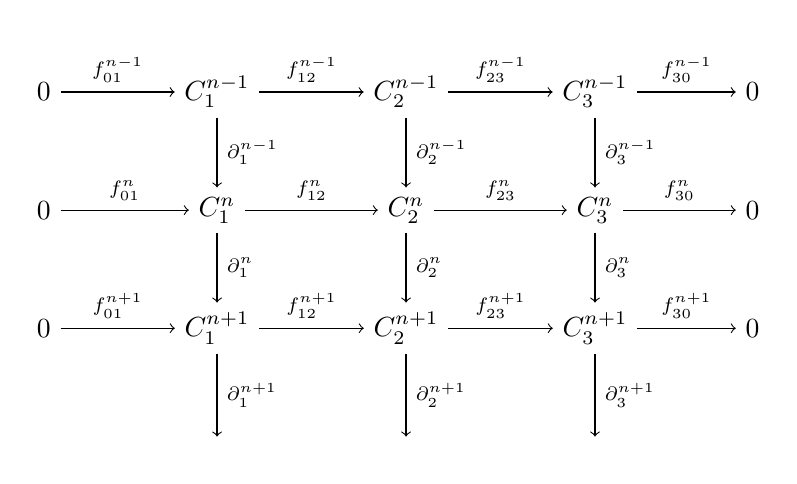
\begin{tikzpicture}[auto]
    %\draw [help lines] (0,0) grid (10,4);%(0,0)から(10,4)までの"細線の方眼"
    \node (hide) at (0,4.2) {};

    \node (0^{n-1}l) at (0,3.5) {$0$};
    \node (C^{n-1}_1) at (2.2,3.5) {$C^{n-1}_1$};
    \node (C^{n-1}_2) at (4.6,3.5) {$C^{n-1}_2$};
    \node (C^{n-1}_3) at (7,3.5) {$C^{n-1}_3$};
    \node (0^{n-1}r) at (9,3.5) {$0$};

    \node (0^nl) at (0,2) {$0$};
    \node (C^n_1) at (2.2,2) {$C^n_1$};
    \node (C^n_2) at (4.6,2) {$C^n_2$};
    \node (C^n_3) at (7,2) {$C^n_3$};
    \node (0^nr) at (9,2) {$0$};

    \node (0^{n+1}l) at (0,0.5) {$0$};
    \node (C^{n+1}_1) at (2.2,0.5) {$C^{n+1}_1$};
    \node (C^{n+1}_2) at (4.6,0.5) {$C^{n+1}_2$};
    \node (C^{n+1}_3) at (7,0.5) {$C^{n+1}_3$};
    \node (0^{n+1}r) at (9,0.5) {$0$};

    \node (0^{n+2}l) at (0,-1) {};
    \node (C^{n+2}_1) at (2.2,-1) {};
    \node (C^{n+2}_2) at (4.6,-1) {};
    \node (C^{n+2}_3) at (7,-1) {};
    \node (0^{n+2}r) at (9,-1) {};

    \draw[->] (0^{n-1}l) to node {$\scriptstyle f_{01}^{n-1}$} (C^{n-1}_1);
    \draw[->] (C^{n-1}_1) to node {$\scriptstyle f_{12}^{n-1}$} (C^{n-1}_2);
    \draw[->] (C^{n-1}_2) to node {$\scriptstyle f_{23}^{n-1}$} (C^{n-1}_3);
    \draw[->] (C^{n-1}_3) to node {$\scriptstyle f_{30}^{n-1}$} (0^{n-1}r);

    \draw[->] (0^nl) to node {$\scriptstyle f_{01}^n$} (C^n_1);
    \draw[->] (C^n_1) to node {$\scriptstyle f_{12}^n$} (C^n_2);
    \draw[->] (C^n_2) to node {$\scriptstyle f_{23}^n$} (C^n_3);
    \draw[->] (C^n_3) to node {$\scriptstyle f_{30}^n$} (0^nr);

    \draw[->] (0^{n+1}l) to node {$\scriptstyle f_{01}^{n+1}$} (C^{n+1}_1);
    \draw[->] (C^{n+1}_1) to node {$\scriptstyle f_{12}^{n+1}$} (C^{n+1}_2);
    \draw[->] (C^{n+1}_2) to node {$\scriptstyle f_{23}^{n+1}$} (C^{n+1}_3);
    \draw[->] (C^{n+1}_3) to node {$\scriptstyle f_{30}^{n+1}$} (0^{n+1}r);

    \draw[->] (C^{n-1}_1) to node {$\scriptstyle \partial^{n-1}_1$} (C^n_1);
    \draw[->] (C^{n-1}_2) to node {$\scriptstyle \partial^{n-1}_2$} (C^n_2);
    \draw[->] (C^{n-1}_3) to node {$\scriptstyle \partial^{n-1}_3$} (C^n_3);

    \draw[->] (C^n_1) to node {$\scriptstyle \partial^n_1$} (C^{n+1}_1);
    \draw[->] (C^n_2) to node {$\scriptstyle \partial^n_2$} (C^{n+1}_2);
    \draw[->] (C^n_3) to node {$\scriptstyle \partial^n_3$} (C^{n+1}_3);

    \draw[->] (C^{n+1}_1) to node {$\scriptstyle \partial^{n+1}_1$} (C^{n+2}_1);
    \draw[->] (C^{n+1}_2) to node {$\scriptstyle \partial^{n+1}_2$} (C^{n+2}_2);
    \draw[->] (C^{n+1}_3) to node {$\scriptstyle \partial^{n+1}_3$} (C^{n+2}_3);
  \end{tikzpicture}
\end{center}
完全列であることから $f_{12}^i$は単射で $f_{23}^i$は全射である。
このとき
\begin{eqnarray*}
  \partial^* : H^n_3 & \longrightarrow & H^{n+1}_1 \\
  \overline{z} = z + B^n_3 & \longmapsto & \overline{x} = x + B^{n+1}_1 := \partial^*(\overline{z})
\end{eqnarray*}
で定まる準同型写像が存在することを示す。
\end{prop}

\begin{proof}
  $(1) \sim (4)$に分けて示す。
  ただし、より一般の完全列に対して $(1) \sim (3)$は蛇の補題から $\partial^* : \ker(\partial^n_3) = Z^n_3 \longrightarrow \coker(\partial^{n+1}_1) = C^{n+1}_1 / B^{n+1}_1$が境界準同型写像の存在性から示される。
  $(1)$では終域が $C^{n+1}_1$よりさらに $Z^{n+1}_1$に狭まることを、
  $(4)$ではとくに $H^n_3 \longrightarrow H^{n+1}_1$で定義できるようになることがさらに示される。

  $(1)$
  以下のような対応 $\partial^*_1$が存在すること
  \begin{eqnarray*}
    \partial^*_1 : Z^n_3 & \longrightarrow & Z^{n+1}_1 \\
    z & \longrightarrow & x
  \end{eqnarray*}
  証明では以下のように元を取っていく。
  \begin{center}
    \begin{tikzpicture}[auto]
      %\draw [help lines] (0,0) grid (10,4);
      \node (x) at (0,0) {$x := (f_{12}^{n+1})^{-1} \circ \partial^n_2(y)$};
      \node (partial^n_2y) at (3.5,0) {$\partial^n_2(y)$};
      \node (y) at (3.5,2) {$y := (f_{23}^n)^{-1}(z)$};
      \node (z) at (6,2) {$z$};
      \node (0r) at (6,0) {$0$};
      \node (0l) at (0,-2) {$0$};

      \draw[->] (z) to node {$\scriptstyle \partial^n_3$} (0r);
      \draw[->] (y) to node {$\scriptstyle f_{23}^n$} (z);
      \draw[->] (y) to node {$\scriptstyle \partial^n_2$} (partial^n_2y);
      \draw[->] (partial^n_2y) to node {$\scriptstyle f_{23}^{n+1}$} (0r);
      \draw[->] (x) to node {$\scriptstyle f_{12}^{n+1}$} (partial^n_2y);
      \draw[->] (x) to node {$\scriptstyle \partial^{n+1}_1$} (0l);
    \end{tikzpicture}
  \end{center}

  $z \in Z^n_3 = \ker(\partial^n) \subset C^n_3$をとる。
  このとき $f_{23}^n$は全射なので $f_{23}^n(y) = z$となる $y \in C^n_2$が少なくとも1つ存在する。
  このうちの一つを $y$としてとると $y = (f_{23}^n)^{-1}(z)$である。
  ここで図式が可換より $\partial^n_3 \circ f_{23}^n = f_{23}^{n+1} \circ \partial^n_2$なので
  $z \in \ker(\partial^n_3)$だから
  $\partial^n_3 \circ f_{23}^n(y) = \partial^n_3(z) = 0$
  なので $f_{23}^{n+1} \circ \partial^n_2(y) = 0$より $\partial^n_2(y) \in \ker(f_{23}^{n+1})$である。
  完全列であることから $\ker(f_{23}^{n+1}) = \im(f_{12}^{n+1})$と
  $f_{12}^{n+1}$は単射だからあるただ一つの $x \in C^{n+1}_1$が存在して
  $f_{12}^{n+1}(x) = \partial^n_2(y)$となるから
  この $x$により $\partial^*(z) := x = (f_{12}^{n+1})^{-1} \circ \partial^n_2 \circ (f_{23}^n)^{-1}(z)$として定めると
  $y = (f_{23}^n)^{-1}(z)$が一つに定まらないことより対応 $\partial^*_1 : Z^n_3 \longrightarrow C^{n+1}_1$が作られる。

  ここで $\partial^{n+1}_1(x) = \partial^{n+1}_1((f_{12}^{n+1})^{-1} \circ \partial^n_2(y))$である。
  図式が可換であることと $f_{12}^i$が単射だから $(f_{12}^{n+1})^{-1} \circ \partial^n_2 = \partial^n_1 \circ (f_{12}^n)^{-1}$より
  $\partial^{n+1} \circ \partial^n = 0$に注意すれば
  $\partial^{n+1}_1(x) = \partial^{n+1}_1((f_{12}^{n+1})^{-1} \circ \partial^n_2(y)) = \partial^{n+1}_1(\partial^n_1 \circ (f_{12}^n)^{-1}(y)) = (\partial^{n+1}_1 \circ \partial^n_1) \circ (f_{12}^n)^{-1}(y) = 0$
  となるから $x \in \ker(\partial^{n+1}_1) = Z^{n+1}_1$となる。
  したがって対応 $\partial^*_1$の終域は $Z^{n+1}_1$となるので上記のような対応が作られる。

  $(2)$
  対応 $\partial^*_1$から以下のような写像 $\partial^*_2$が作られること
  \begin{eqnarray*}
    \partial^*_2 : Z^n_3 & \longrightarrow & H^{n+1}_1 (:= Z^{n+1}_1 / B^{n+1}_1) \\
    z & \longrightarrow & \overline{\partial^*_1(z)} = \overline{x} = x + B^{n+1}_1
  \end{eqnarray*}
  いま $\partial^*_1$によって $z = z' \in Z^n_3$に対し、ある $y = (f_{23}^n)^{-1}(z) , y' = (f_{23}^n)^{-1}(z')$は $y \neq y'$になる可能性がある。
  その $y , y'$に対しては $\partial^n_2$が写像で $f_{12}^n$が単射より
  ただ一つの $x = (f_{12}^{n+1})^{-1} \circ \partial^n_2(y) , x' = (f_{12}^{n+1})^{-1} \circ \partial^n_2(y')$が存在する。
  このとき $x - x' \in B^{n+1}_1$であれば $\overline{x} = \overline{x'}$となるから $\partial^*_2$が写像になる。
  したがって $x - x' \in B^{n+1}_1$を示せばいい。

  以下のような可換性を用いる。
  \begin{center}
    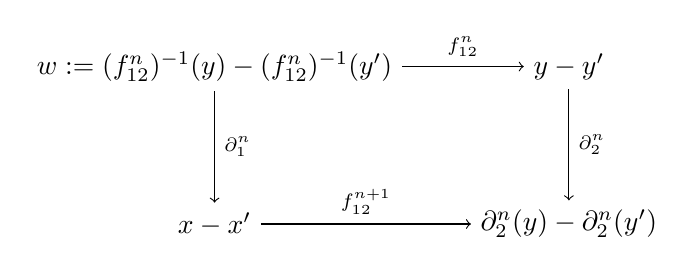
\begin{tikzpicture}[auto]
      %\draw [help lines] (0,0) grid (10,4);
      \node (x-x') at (0,0) {$x - x'$};
      \node (w) at (0,2) {$w := (f_{12}^n)^{-1}(y) - (f_{12}^n)^{-1}(y')$};
      \node (partial^n_2y - partial^n_2y') at (4.5,0) {$\partial^n_2(y) - \partial^n_2(y')$};
      \node (y-y') at (4.5,2) {$y - y'$};

      \draw[->] (y-y') to node {$\scriptstyle \partial^n_2$} (partial^n_2y - partial^n_2y');
      \draw[->] (w) to node {$\scriptstyle \partial^n_1$} (x-x');
      \draw[->] (x-x') to node {$\scriptstyle f_{12}^{n+1}$} (partial^n_2y - partial^n_2y');
      \draw[->] (w) to node {$\scriptstyle f_{12}^n$} (y-y');
    \end{tikzpicture}
  \end{center}

  $x - x' = (f_{12}^{n+1})^{-1} \circ \partial^n_2(y) - (f_{12}^{n+1})^{-1} \circ \partial^n_2(y')$である。
  $f_{12}^i$が単射で図式が可換より $(f_{12}^{n+1})^{-1} \circ \partial^n_2 = \partial^n_1 \circ (f_{12}^n)^{-1}$となる。
  よって $\partial^n_1$が準同型だから $x - x' = \partial^n_1 \circ (f_{12}^n)^{-1}(y) - \partial^n_1 \circ (f_{12}^n)^{-1}(y') = \partial^n_1((f_{12}^n)^{-1}(y) - (f_{12}^n)^{-1}(y'))$となる。
  ここで $w := (f_{12}^n)^{-1}(y) - (f_{12}^n)^{-1}(y') \in C^n_1$より
  $x - x' = \partial^n_1(w) \in \im(\partial^n_1) = B^{n+1}_1$より示された。

  とくに、以上のことから $\partial^*_2$は $y = (f_{23}^n)^{-1}(z)$のとり方によらないので以下ではある一つを任意に取ることとする。

  $(3)$
  写像$\partial^*_2$が準同型になること

  $\partial^*_2(z) = \overline{x} , \partial^*_2(z') = \overline{x'} , x = (f_{12}^{n+1})^{-1} \circ \partial^n_2(y) , x' = (f_{12}^{n+1})^{-1} \circ \partial^n_2(y')$とする。
  ここで $f_{23}^n$が準同型より
  $f_{23}^n(y + y') = f_{23}^n(y) + f_{23}^n(y') = z + z'$だから
  $y + y' = (f_{23}^n)^{-1}(z + z')$となる。
  また、 $f_{12}^{n+1} , \partial^n_2$が準同型より
  $f_{12}^{n+1}(x + x') = f_{12}^{n+1}(x) + f_{12}^{n+1}(x') = \partial^n_2(y) + \partial^n_2(y') = \partial^n_2(y + y')$なので
  $x + x' = (f_{12}^{n+1})^{-1} \circ \partial^n_2(y + y')$とできる。
  以上より $\partial^*_2(z + z') = \overline{x + x'} = x + x' + B^{n+1}_1 = (x + B^{n+1}_1) + (x' + B^{n+1}_1) = \overline{x} + \overline{x'} = \partial^*_2(z) + \partial^*_2(z')$となるから $\partial^*_2$は準同型になる。

  $(4)$
  準同型写像 $\partial^*_2$から以下のような準同型写像 $\partial^*$が誘導されること。
  \begin{eqnarray*}
    \partial^* : H^n_3 & \longrightarrow & H^{n+1}_1 \\
    \overline{z} = z + B^n_3 & \longmapsto & \partial^*_2(z) = \overline{x} = x + B^{n+1}_1
  \end{eqnarray*}
  以下のような可換性を用いる。
  \begin{center}
    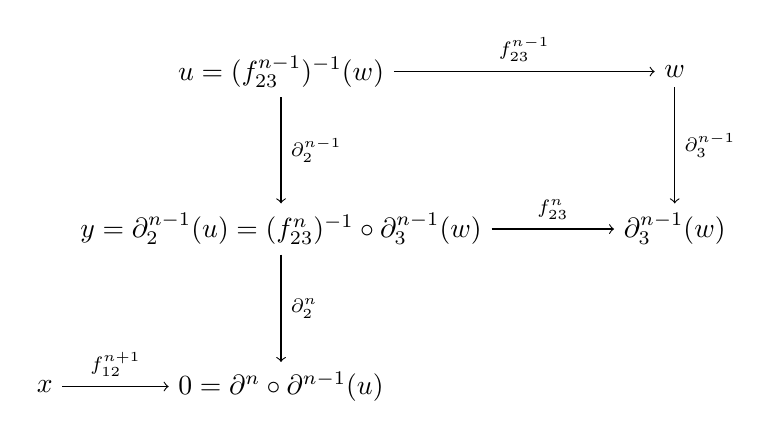
\begin{tikzpicture}[auto]
      %\draw [help lines] (0,0) grid (10,4);
      \node (x) at (0,0) {$x$};
      \node (y) at (3,2) {$y = \partial^{n-1}_2(u) = (f_{23}^n)^{-1} \circ \partial^{n-1}_3(w)$};
      \node (u) at (3,4) {$u = (f_{23}^{n-1})^{-1}(w)$};
      \node (w) at (8,4) {$w$};
      \node (partial^{n-1}_3w) at (8,2) {$\partial^{n-1}_3(w)$};
      \node (0) at (3,0) {$0 = \partial^n \circ \partial^{n-1}(u)$};

      \draw[->] (w) to node {$\scriptstyle \partial^{n-1}_3$} (partial^{n-1}_3w);
      \draw[->] (u) to node {$\scriptstyle f_{23}^{n-1}$} (w);
      \draw[->] (u) to node {$\scriptstyle \partial^{n-1}_2$} (y);
      \draw[->] (y) to node {$\scriptstyle f_{23}^n$} (partial^{n-1}_3w);
      \draw[->] (y) to node {$\scriptstyle \partial^n_2$} (0);
      \draw[->] (x) to node {$\scriptstyle f_{12}^{n+1}$} (0);
    \end{tikzpicture}
  \end{center}

  $\partial^*_2$はすでに準同型写像なので $\partial^*(\overline{z}) = \partial^*_2(z + B^n_3)$より $\partial^*_2(B^n_3) = 0$となれば
  $\partial^*(\overline{z}) = \partial^*_2(z) = \overline{x}$とできて準同型写像が誘導される。
  したがって $\partial^*_2(B^n_3) = 0$を示す。

  $B^n_3 = \im(\partial^{n-1}_3)$より $B^n_3$の元は
  任意の $w \in C^{n-1}_3$を用いて $\partial^{n-1}_3(w)$で書かれる。
  $\partial^n \circ \partial^{n-1} = 0$より $B^n_3 \im(\partial^{n-1}_3) \subset \ker(\partial^n_3) = Z^n_3$なので $\partial^*_2$の定義域に即している。
  この $\partial^{n-1}_3(w)$に対して今までと同様に
  $y = (f_{23}^n)^{-1}(\partial^{n-1}_3(w))$と
  $x = (f_{12}^{n+1})^{-1} \circ \partial^n_2(y)$が取れる。
  ここで $f_{23}^{n-1}$が全射なので $f_{23}^{n-1}(u) = w$となる $u \in C^{n-1}_2$が存在する。
  図式が可換より $\partial^{n-1}_3 \circ f_{23}^{n-1}(u) = f_{23}^n \circ \partial^{n-1}_2(u)$であるので
  $\partial^{n-1}_3(w) = f_{23}^n \circ \partial^{n-1}_2(u)$から
  $\partial^{n-1}_2(u) = (f_{23}^n)^{-1} \circ \partial^{n-1}_3(w) = y$
  となる。
  これより $\partial^n_2 \circ \partial^{n-1}_2 = 0$に注意すれば
  $\partial^*_2(\partial^{n-1}_3(w)) = (f_{12}^{n+1})^{-1} \circ \partial^n_2(y) = (f_{12}^{n+1})^{-1} \circ (\partial^n_2 \circ \partial^{n-1}_2)(u) = 0$
  となるので $\partial^{n-1}_3(w) \in \ker(\partial^*_2)$より
  $\partial^*_2(B^n_3) = 0$から適切に $\partial^*$が誘導される。

  以上より準同型写像 $\partial^* : H^n_3 \longrightarrow H^{n+1}_1 , \overline{z} \longmapsto \overline{x}$が存在することが示された。
\end{proof}

\begin{fact}
  $G$加群 $M_i (1 \leq i \leq 3)$に対して以下の加群の完全列が存在するとする。
  \begin{eqnarray*}
    0 \longrightarrow M_1 \longrightarrow M_2 \longrightarrow M_3 \longrightarrow 0
  \end{eqnarray*}
  このとき以下のような無限の長さの完全列が存在する。
  \begin{eqnarray*}
    0 & \longrightarrow & H^0(G,M_1) \longrightarrow H^0(G,M_2) \longrightarrow H^0(G,M_3) \\
    & \longrightarrow & H^1(G,M_1) \longrightarrow H^1(G,M_2) \longrightarrow H^1(G,M_3) \\
    & \longrightarrow & H^2(G,M_1) \longrightarrow \cdots
  \end{eqnarray*}
\end{fact}

\subsection{Galois cohomology}

\begin{defi}
  $A$を群 $G$が作用する\rm{Abel}とは限らない群とする。
  このとき例 $(\mathrm{\ref{exam:cohomology0}})$より
  $0$次のコホモロジー群を
  $H^0(G,A) := A^G$としても矛盾しないのでそのように定義する。

  また、 $\alpha \in C^1(G,A)$を
  \begin{eqnarray*}
    \alpha : G & \longrightarrow & A \\
    g & \longmapsto & \alpha_g
  \end{eqnarray*}
  と定めると、 $A$の演算を非可換性を表すため積で書くことにすると
  \begin{eqnarray*}
    \partial^1(\alpha)(g , h) & = & g \alpha_h \cdot \alpha_{gh}^{-1} \cdot \alpha_g \\
    \alpha \in Z^1 = \ker(\partial^1) & \Leftrightarrow & {}^\forall g , h \in G , g \alpha_h \cdot \alpha_{gh}^{-1} \cdot \alpha_g = 1 \\
    & \Leftrightarrow & \alpha_{gh}^{-1} \cdot \alpha_g = (g \alpha_h)^{-1} \\
    & \Leftrightarrow & \alpha_g (g \alpha_h) = \alpha_{gh}
  \end{eqnarray*}
  となるから
  例 $(\mathrm{\ref{exam:cohomology1}})$より
  $1$次のコサイクルは
  $Z^1 = \{ \alpha \in C^1 | {}^\forall g , h \in G , \alpha_{gh} = \alpha_g \cdot g \alpha_h \}$
  となるのでそのように定義する。
\end{defi}

\begin{defi}
  群 $G$とそれが作用する非可換群 $A$の
  $1$次コサイクル $Z^1$について
  $\alpha , \beta \in Z^1$が\underline{\rm{cohomologous}} $(\alpha \sim \beta)$とは
  \[
  {}^\exists a \in A \  \mathrm{s.t.} \
  {}^\forall g \in G \  , \  \beta_g = a^{-1} \cdot \alpha_g \cdot ga
  \]
  となることであり、これは同値関係になる。
  $G$が恒等的な作用をするのであれば $ga = a$より
  これは $\alpha_g$と $\beta_g$が共役な関係になってることと同じになる。
  つまり共役から $ga$の分だけねじれているともみれる。
\end{defi}

\begin{proof}
  同値関係になることをしめす。

  まず、 ${}^\forall g \in G$と ${}^\forall a \in A$について
  $(ga)^{-1} = ga^{-1} , g(1) = 1$が成り立つことを示す。
  定義から $G$が $A$に加群のように作用するので
  $g(1) = g(1 \cdot 1) = g(1) \cdot g(1)$から
  $g(1) = g(1) \cdot g(1)^{-1} = 1$より成立。
  これを用いれば $1 = g(1) = g(a \cdot a^{-1}) = ga \cdot ga^{-1} \Leftrightarrow (ga)^{-1} = ga^{-1}$より成立。

  ・反射律

  $a = 1 \in A$としてとれば
  $\alpha_g = 1 \cdot \alpha_g \cdot 1 = 1^{-1} \cdot \alpha_g \cdot g(1)$
  が任意の $g \in G$で成り立つので $\alpha \sim \alpha$より反射律が成り立つ。

  ・対称律

  $\alpha \sim \beta$のときある $a \in A$で $\beta_g = a^{-1} \cdot \alpha_g \cdot ga$となっているので逆元をそれぞれかけて
  $\alpha_g = a \cdot \beta_g \cdot (ga)^{-1}$となっていて
  上で述べたことより $b := a^{-1} \in A$を取る時 $(ga)^{-1} = ga^{-1} = gb$から
  $\alpha_g = b^{-1} \cdot \beta_g \cdot gb$となるので $\beta \sim \alpha$より対称律がなりたつ。

  ・推移律

  $\alpha \sim \beta , \beta \sim \gamma$となっているとするとき
  ある $a , b \in A$で $\beta_g = a^{-1} \cdot \alpha_g \cdot ga$と
  $\gamma_g = b^{-1} \cdot \beta_g \cdot gb$となっている。
  $\beta_g$に代入すると $\gamma_g = b^{-1} \cdot (a^{-1} \cdot \alpha_g \cdot ga) \cdot gb = (b^{-1} a^{-1}) \cdot \alpha_g \cdot (ga \cdot gb) = (ab)^{-1} \cdot \alpha_g \cdot g(ab)$となり
  $ab \in A$なので $\alpha \sim \gamma$から推移律が成り立つ。
\end{proof}

\begin{defi}
  \rm{Galois cohomology}とは有限次\rm{Galois}拡大 $L/K$があるとき
  $G := \gal(L/K)$としてこれが作用する群 $M$についての
  コホモロジー群 $H^n(G,M)$のことである。
  とくに $M$として $L , L^n , GL_n(L)$等を考える。
  ただし $GL_n(L)$は $L$成分の $n$次正則行列全体の積による群であり、
  一般に $L$に作用する群を $G$としたとき $\sigma \in G$は $X = (x_{ij}) \in M_n(L) := (n次正方行列全体の集合)$に対して
  $\sigma(X) := (\sigma(x_{ij}))$と定める。
\end{defi}

\begin{prop}
  体 $L$と有限群 $G \subset \aut(L)$について以下が成り立つ。

  $(1)$
  ${}^\forall n \in \Z_{\geq 1}$について
  $H^n(G,L) = 0$となる。

  $(2)$
  ${}^\forall n \in \Z_{\geq 1}$について
  $H^1(G,GL_n(L)) = 1$となる。
  とくに $H^1(G,L^\times) = 1$となる。
  これは一つの成分だけの正則行列が $GL_1(L) = L^\times$となることからすぐ導かれる。
\end{prop}

\begin{proof}
  $(2)$

  一般に定義 $(\mathrm{\ref{defi:cohomology}})$から $B^1 \subset Z^1$だから
  $Z^1 \subset B^1$を示せば $B^1 = Z^1$から $H^1 = Z^1/B^1 = 1$が示される。
  まず、 $0$次コバウンダリー作用素 $\partial^0$に対して
  $B^1 = \im(\partial^0) = \{ \partial^0 X | X \in GL_n(L) \}$となっていて
  例 $(\mathrm{\ref{exam:cohomology1}})$の $B^1$から
  $\partial^0 X$は $GL_n(L)$での演算は積であることに注意すれば
  \begin{eqnarray*}
    \partial^0 X : G & \longrightarrow & GL_n(L) \\
    g & \longmapsto & \partial^0 X(g) = gX \cdot X^{-1}
  \end{eqnarray*}
  となっている。
  したがって ${}^\forall \alpha \in Z^1$に対して
  ${}^\forall g \in G , \alpha_g = \partial^0 X(g) = gX \cdot X^{-1}$となる
  $X \in GL_n(L)$が存在すればよい。
  いま、ある $X \in GL_n(L)$について
  \begin{eqnarray*}
    b := \sum_{h \in G} \alpha_h \cdot h(X)
  \end{eqnarray*}
  と定義すると $b \in GL_n(L)$である。
  $h \in G \subset \aut(L)$より\rm{Dedekind}の補題 $(\mathrm{\ref{lemm:dedekind}})$から $M$を $L$とみれば
  その対偶を取ることで
  $\alpha_h \in GL_n(L)$はより任意の $h \in G$で $\alpha_h \neq 0$となるから
  ある $x_{ij} \in L$が存在して $\sum_{h \in G} \alpha_h \cdot hx_{ij} \neq 0$
  となる。
\end{proof}

\end{document}
